\documentclass[a4paper,11pt]{jsarticle}
\usepackage{amsmath, amsfonts}
\usepackage{bm}
\usepackage[dvipdfmx]{graphicx}
\usepackage{here}
\newcommand{\ywx}{y_i{\bm w}^\top{\bm x}_i}
\renewcommand{\exp}[1]{\text{exp}\left({#1}\right)}
\begin{document}
  \title{先端データ解析論 大レポート}
  \author{情報理工学系研究科電子情報学専攻M1 堀 紡希 48216444}
  \date{\today}
  \maketitle
  各課題を実装したipynbファイルもこのファイルと一緒に提出する。
  \section*{1}
  比較のために、通常のニューラルネットワークでのMNIST分類lossの推移を示す。
  \begin{figure}[H]
    \centering
    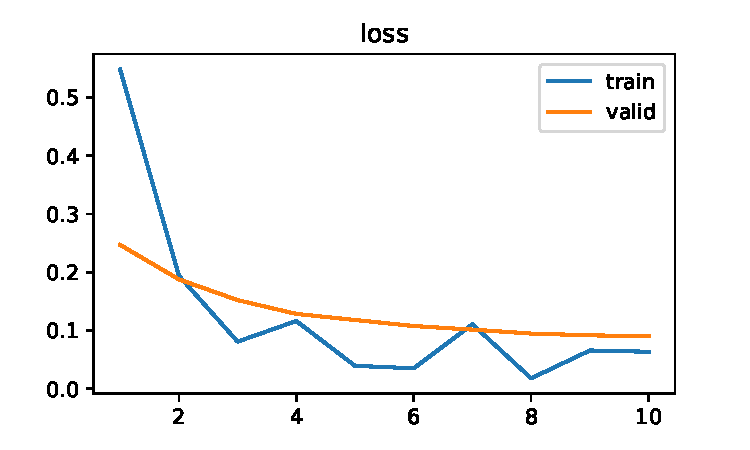
\includegraphics[width=0.6\linewidth]{ortho.pdf}
    \caption{通常のニューラルネットワークでのMNIST分類のlossのepoch数に伴う変化。}
  \end{figure}

  \subsection*{早期打ち切り}
  早期打ち切りを実装した。
  20epoch繰り返したところ13epochで検証データのlossが最小になり、これ以上は汎化性能は上がらないと考え、この時点でのモデルを採用することになる。
  \begin{figure}[H]
    \centering
    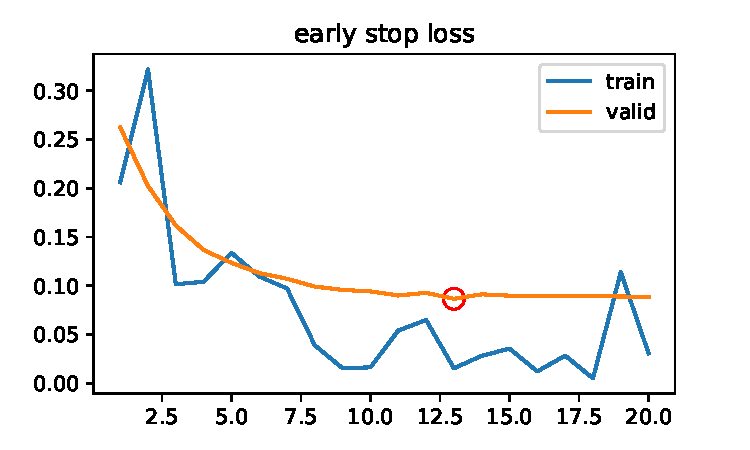
\includegraphics[width=0.6\linewidth]{earlystop.pdf}
    \caption{早期打ち切りでのMNIST分類のlossのepoch数に伴う変化。赤丸の時点でlossが最小になっている。}
  \end{figure}

  \subsection*{ラベル平滑化}
  ラベル平滑化を実装した(ハイパーパラメータは0.2)。
  損失関数の値が大きくなるため、当然だがlossの値が大きくなっている。1回目のepochで顕著だが、検証データと訓練データのlossの差が小さくなっている。
  これは正則化の作用によるものと考えることが出来る。
  \begin{figure}[H]
    \centering
    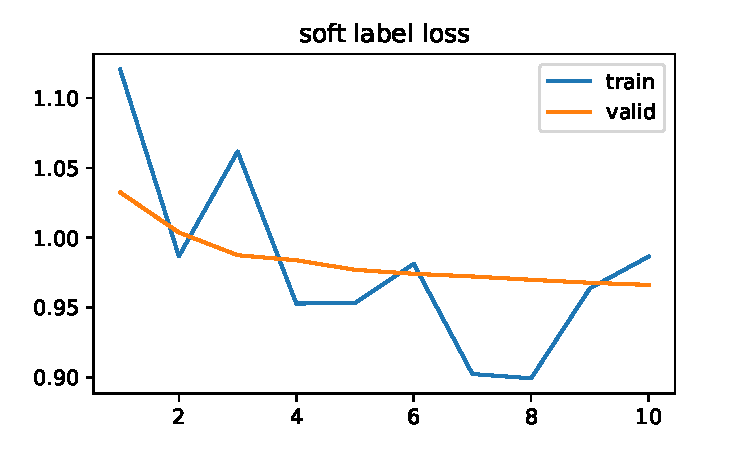
\includegraphics[width=0.6\linewidth]{softlabel.pdf}
    \caption{ラベル平滑化を施したMNIST分類のlossのepoch数に伴う変化。}
  \end{figure}

  \subsection*{dropout}
  dropoutを実装した(ハイパーパラメータは0.2)。
  中間層に0.2のdropoutを追加した。確率的に学習を止めるため訓練データのlossが変動が大きくなっているが、検証データのlossは一貫して小さくなっている。
  \begin{figure}[H]
    \centering
    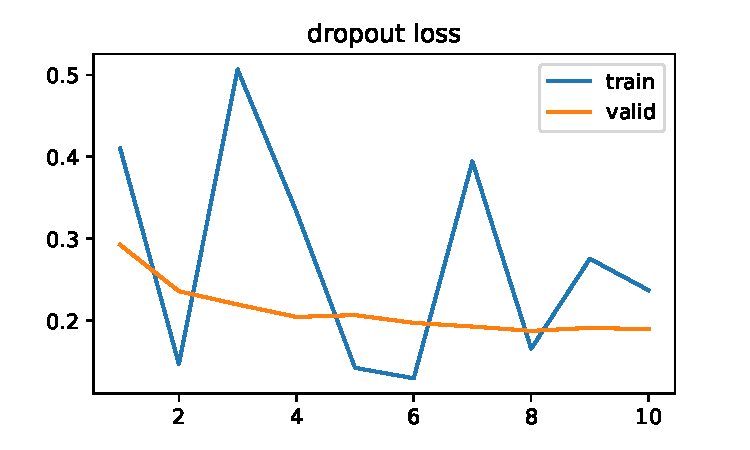
\includegraphics[width=0.6\linewidth]{dropout.pdf}
    \caption{dropoutを施したMNIST分類のlossのepoch数に伴う変化。}
  \end{figure}



  \section*{2}
  隠れ層一層の自己符号化器を実装した。この自己符号化器の作用により、雑音を加えられたMNISTのデータ(上段)から
  雑音を取り除いたデータ(下段)が生成されている。
  \begin{figure}[H]
    \centering
    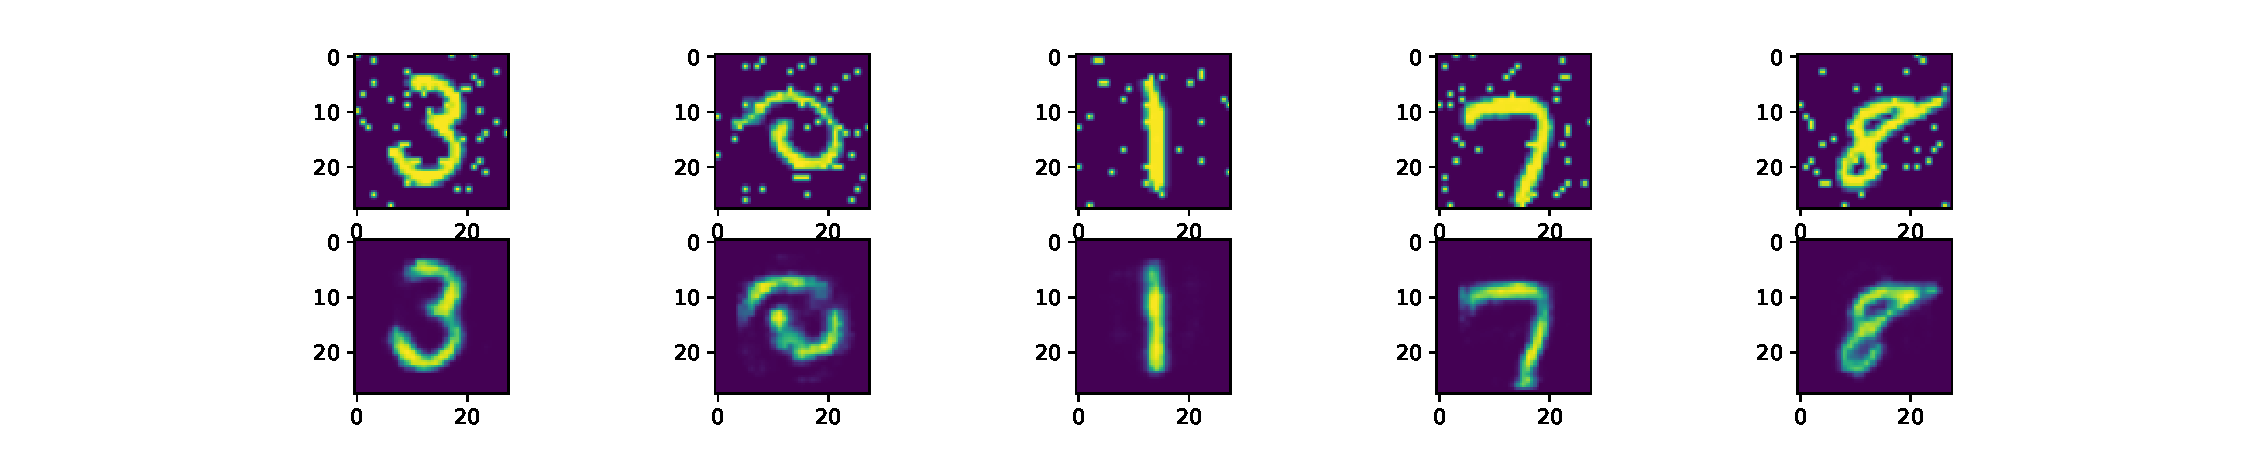
\includegraphics[width=\linewidth]{../autoencoder.pdf}
    \caption{雑音を加えたMNISTのデータから自己符号化器によってノイズを除去した図}
  \end{figure}

\end{document}